\chapter{Method}\label{cha:method}

This paper present a algorithm to detect facial marks automatically. This section will describe the methods briefly used to develop the algorithm. If more details are requested, they can be found in the referred works. 

\section{Detection}

An overview of the detections system is presented in figure \ref{fig:detection_flow}. The system consist of several subsystems which has it own functionality. Each image, \textit{I}, is processed and go through each of these subsystems. 

\subsection{Face detection}

An important component for further processing is the bounding box of the face in each image. It is found by using an implementation of object detection by Paul Viola et al. \cite{face_detection}. The algorithm take advantage of three different parts. 

The first is part is a new image representation which allows Haar features from each image to be calculated rapidly. The speed is achieved by using integral images instead of the original image. 

The second part is the extraction of the most important features through AdaBoosting. It creates a strong classifier by combining the strength of weaker classifiers. A weak classifier is the best threshold for a feature which separates the faces from the non-faces.

The third part is a cascade decision which reduces the computations costs by rejecting potential bounding boxes for the face. If the first weak classifier gives a positive result, the second classifier is engaged. This is repeated until all weak classifiers has been passed or if one of the returns a negative result. All bounding boxes which has returned a negative result is rejected immediately.  

When a suitable bonding box as been found for \textit{I}, the landmarks in the image can be extracted. 

\subsection{Landmark detection}

With landmark in the face, it is possible to create a unique mask for each face and produce a grid with different regions in the face. The landmarks are extracted by using an implantation based on Vahid Kazemi et al.\cite{dlib_landmark} It uses sate of the art algorithms for face alignment where cascade of regression functions are crucial for its success. The estimated shape of the face is updated by regressing the shape parameters based on normalized features from the image. The parameters are updated until they converges.  

From this algorithm, 68 landmarks are extracted where the eyes, moth, nose and chin are marked. From these, a mask generated where the nostrils, eyes, throat and background is cut out. Also, a grid of 16 regions is generated according to the supervisors at NFC demands. 

\subsection{Normalization}

In order to get a reliable and uniform result, the image has to be normalized. There are two kind of normalization applied on the image, geometric normalization and photometric normalization.  

The geometric normalization consist of rotation of the image such that the eyes are aligned with the bottom of the image. The rotations angle is calculated with the help of the landmarks at the corners of the eyes. An angle is calculated by averaging an angle from the right and left eye. The geometric normalization also include a resize of the image such that the interpupillary distance is 500 pixels. A resizing factor is calculated by taking the fraction between 500 and the distance between the pupils.         

The photometric normalization is performed by using tone mapping operator based on the work of Nikola Banic et al.\cite{badger}. It uses a Light Random Sprays Retinex (LRSR) which is an improvement of the Random Sprays Retinex (RSR)\cite{RSR}. All tone mapping operator transform pixel intensities depending on its surrounding and the RSR uses a random selection of pixels around the the current pixel which decreases computations costs, sampling noise and dependency. The calculations are done on intensity image for LRSR while uses the RGB colour channels.
         
\subsection{Segmentation}

When searching for facial mark, hair lines and hair can cause false detection. Therefore the image has to be segmented so that only skin area is regarded in search for facial marks. The segmentation is done with GrabCut produced by Carsten Rother et al.\cite{grabcut}. It uses Gaussian Mixture Model (GMM) for a colour image. GrabCut needs a GMM for know foreground and one for known background. The known foreground used e.g. is the cheeks and forehead, which is extracted from the landmarks. 

After creating GMM:s, a energy function is created so that its minimum correspond to a good segmentation which depends on the given foreground and background. The function is minimized iteratively until a converged segmentation is produced.

The segmentation mask is used to improve the mask created from the landmarks. Now using the improved mask, a well segmented image can searched for facial marks. This image will henceforth be called \textit{$I_{pre}$}

\subsection{Colour space}

Facial marks tend to have a brown or red colour and thus would it be of interest to process these colours in the image. This is possible by converting the RGB image to red-channel and brown-channel images respectively. This is done by using a trained transformer from the work of Joost van de Weijer et al.\cite{11_colours}. It is trained on real world images from Google Image and has shown to out perform colour chips. The colour transformed images are used for the watershed algorithm to find the contours of the facial marks and to extract relevant features for the classifier. 


\subsection{Fast Radial Symmetry Detector}

The actual mark detection uses local radial symmetry to detect interesting point in the \textit{$I_{pre}$}. The algorithm used i called Fast Radial Symmetry and was created by Gareth Loy et al.\cite{FRS}. For each point, $p$, in the \textit{$I_{pre}$}, the contribution of radial symmetry at radius $r$ is calculated by producing a orientation projection image $O_n$ and a magnitude projection image $M_n$. These images are created by examining the positively-affected, $p_{+}(p)$, and negatively-affected, $p_{-}(p)$. To do this, the gradient, $g$, of the image is needed and it is calculated using a 3x3-Sobel kernel. Since the gradient computations are discrete, it is necessary to average \textit{$I_{pre}$} with a 3x3 Gaussian kernel to remove sharp edges. 

\begin{equation} \label{eq:p+}
p_{+}(p) = g(p) + round\frac{g(p)}{\norm{g(p)}}n
\end{equation}

\begin{equation} \label{eq:p-}
p_{-}(p) = g(p) - round\frac{g(p)}{\norm{g(p)}}n
\end{equation}

The $O_n$ and $M_n$ are then updated according to \cref{eq:O+,eq:O-,eq:M+,eq:M-}

\begin{equation} \label{eq:O+}
O_{n}(p_{+}) = O_{n}(p_{+}) + 1
\end{equation}
\begin{equation} \label{eq:O-}
O_{n}(p_{-}) = O_{n}(p_{-}) - 1
\end{equation}
\begin{equation} \label{eq:M+}
M_{n}(p_{-}) = M_{n}(p_{+}) + \norm{g(p)}
\end{equation}
\begin{equation} \label{eq:M-}
M_{n}(p_{-}) = M_{n}(p_{-}) - \norm{g(p)}
\end{equation}

The radial symmetry contribution at radius n depends on $F_n$ and $A_n$ which is defined as 

\begin{equation} \label{eq:F}
F_n = \frac{M_{n}(p)}{k_n} \left(\frac{\abs{\tilde{O}_n(p)}}{k_n}\right)^{\alpha}
\end{equation}
\begin{equation} \label{eq:A}
 \tilde{O}_n(p) =   
 \begin{cases}
 O_n(p)    & \quad \text{if } O_n(p) < k_n\\
 0		& \quad  \text{ else}\\
 \end{cases}
\end{equation}

$A_n$ is a Gaussian kernel with different size depending on $n$, $\alpha$ is radial strictness parameter and $k_n$ is a scaling factor. $\alpha$ is set to $2$ and $k_n$ to $9.9$ since Gareth Loy et al. deemed suitable for most applications.

The final radial symmetry image $S_n$ is calculate 

\begin{equation} \label{eq:M-}
S_{n} = F_n * A_n
\end{equation}

This was a calculation for radius $n$ and it desirables to use multiple radii to detect point larger then $n$. It is not necessary to use a continuous spectrum of radii, thus the radii used are $N = \{1, 3, 5, 7, 9, 11, 13, 15 \}$

The average of radial symmetry images, $S$, are calculated as

\begin{equation} \label{eq:M-}
S =\frac{1}{N} \sum_{n=1}^{N} S_n
\end{equation}

At this point, a image with points of interest has been acquired. From this image, a binary threshold was applied with the threshold $h_{FRS}$ to extract sinks for the watershed algorithm described by Fernand Meyer \cite{watershed}. The output is now a set of bonding boxed containing facial mark candidates.

\subsection{Candidate elimination}

Since many facial mark candidates may be false positives, they have to be discovered and excluded. Each candidate is given a 25x25 area which is processed through two eliminators. 

The first eliminator uses a simple blob detector. It searched thresholded binary images for connective pixels and returns true is the area contains a blob. If the mark does not contain a blob, it is excluded from the candidates.   

The eliminator uses a hair removal algorithm by Tim Lee et. al.\cite{dullrazor}. The algorithm smooth out hair pixels with closing operations using the three different structuring elements. The suggested structuring elements by Tim Lee et. al. is $T_{0}$, $T_{45}$ and $T_{90}$. \\

$T_{0} =
\left[ \begin{array}{@{}*{13}{c}@{}}
0 & 1 & 1 & 1 & 1 & 1 & 1 & 1 & 1 & 1 & 1 & 1 & 0  \\
\end{array} \right]  $ \\

$T_{45} =
\left[ \begin{array}{@{}*{9}{c}@{}}
0 & 0 & 0 & 0 & 0 & 0 & 0 & 0 & 0 \\
0 & 1 & 0 & 0 & 0 & 0 & 0 & 0 & 0 \\
0 & 0 & 1 & 0 & 0 & 0 & 0 & 0 & 0 \\
0 & 0 & 0 & 1 & 0 & 0 & 0 & 0 & 0 \\
0 & 0 & 0 & 0 & 1 & 0 & 0 & 0 & 0 \\
0 & 0 & 0 & 0 & 0 & 1 & 0 & 0 & 0 \\
0 & 0 & 0 & 0 & 0 & 0 & 1 & 0 & 0 \\
0 & 0 & 0 & 0 & 0 & 0 & 0 & 1 & 0 \\
0 & 0 & 0 & 0 & 0 & 0 & 0 & 0 & 0 \\
\end{array} \right]$ \\

$T_{90} = (T_{90})^{T} $ \\


The closed image is generated by applying each structure element on each colour channel as \ref{eq:hair}, where $G$ is the closed image, $M$ is the image of a mark, $T_x = [T_{0}, T_{45}, T_{90} ]$ and $C$ the RGB-channels.

\begin{equation} \label{eq:hair}
G_c = \abs{M_c - max(M_c * T_x)}
\end{equation}

If the number of hair pixels in the union of $G_c$ is larger then a threshold $h_{hair}$, the mark is excluded from the candidates.  


\begin{figure}[tbp]
  \centering
  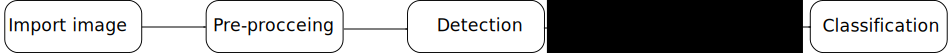
\includegraphics{detection_flow}
  \caption{\label{fig:detection_flow}%
  }
\end{figure}

\section{Classification}

The algorithm should also separate RPPVSM from non-permanent marks. This is done by training a SVM-classifiers using radial basis function kernels and 1000 iteration. The training data consists of the labelled facial marks provided by the supervisors at NFC. To get a good classifier, a set of features are required. 

\subsection{Features}
The features extracted from the facial marks can be looked up in the table below. 

\begin{center}
	\begin{tabular}{|l|p{9cm}|}
	\hline
	Feature & Description	\\ \hline
	Mean & Mena from RGB channels and red and brown channel \\ \hline
	Standard deviation & Standard deviation from RGB channels and red and brown channel	\\ \hline
	\end{tabular}
\end{center}


\section{Experiment}
